\documentclass[tikz,border=1pt]{standalone}
\usepackage{tikz}
\usepackage{amsmath}
\usetikzlibrary{trees,positioning}

\begin{document}
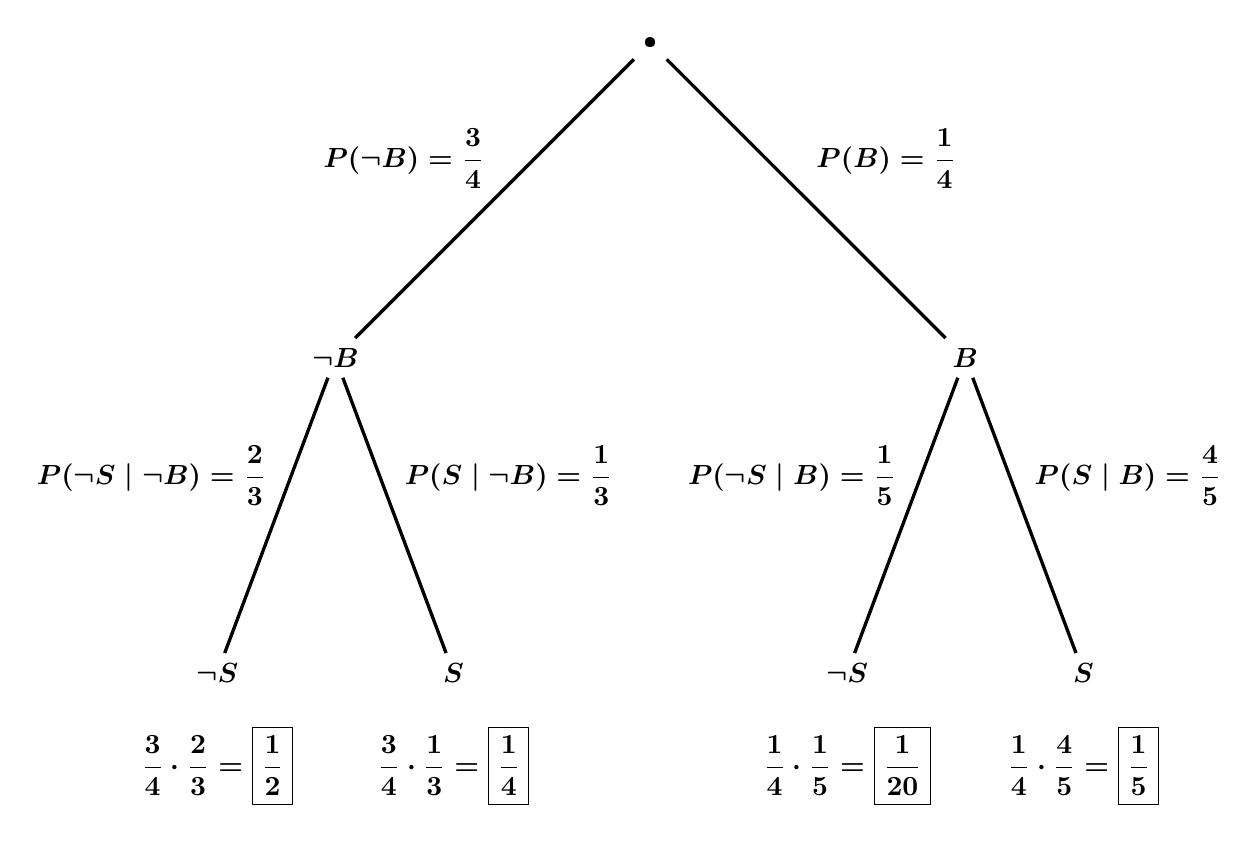
\begin{tikzpicture}[
    level distance=40mm,
    sibling distance=50mm,
    edge from parent/.style={draw, -, very thick},
    every node/.style={thick}
    ]
    \boldmath
    \node (root) {\textbullet} [sibling distance=80mm]
    child { node (nB) {$\lnot B$} [sibling distance=30mm]
        child { node (nSnB) {$\lnot S$} 
          edge from parent node[above left]{$P(\lnot S\mid\lnot B)=\dfrac{2}{3}$}
        }
        child { node (SnB) {$S$}
          edge from parent node[above right]{$P(S\mid\lnot B)=\dfrac{1}{3}$}
        }
        edge from parent node[above left]{$P(\lnot B)=\dfrac{3}{4}$}
    }
    child { node (B) {$B$} [sibling distance=30mm]
        child { node (nSB) {$\lnot S$}
          edge from parent node[above left]{$P(\lnot S\mid B)=\dfrac{1}{5}$}
        }
        child { node (SB) {$S$}
          edge from parent node[above right]{$P(S\mid B)=\dfrac{4}{5}$}
        }
        edge from parent node[above right]{$P(B)=\dfrac{1}{4}$}
    };
    
    \node[below=3mm of nSnB]   {$\dfrac{3}{4}\cdot\dfrac{2}{3}=\boxed{\dfrac{1}{2}}$};
    \node[below=3mm of SnB]    {$\dfrac{3}{4}\cdot\dfrac{1}{3}=\boxed{\dfrac{1}{4}}$};
    \node[below=3mm of nSB]    {$\dfrac{1}{4}\cdot\dfrac{1}{5}=\boxed{\dfrac{1}{20}}$};
    \node[below=3mm of SB]     {$\dfrac{1}{4}\cdot\dfrac{4}{5}=\boxed{\dfrac{1}{5}}$};
\end{tikzpicture}
\end{document}
